% ============================================================
% Real-Time Traffic Analytics Pipeline -- Group 13
% Works with pdfLaTeX (default on Overleaf) as well as XeLaTeX / LuaLaTeX.
% ============================================================
\documentclass[12pt,a4paper]{article}

% ------------------------------------------------------------
% Packages
% ------------------------------------------------------------
\usepackage{iftex}
\ifPDFTeX
  % pdfLaTeX: Vietnamese support through the T5 encoding
  \usepackage[utf8]{inputenc}
  \usepackage[T5]{fontenc}
  \usepackage{lmodern}
\else
  % XeLaTeX / LuaLaTeX
  \usepackage{fontspec}
  \setmainfont{Latin Modern Roman}
  \setsansfont{Latin Modern Sans}
  \setmonofont{Latin Modern Mono}
\fi
\usepackage[margin=2.5cm]{geometry}
\usepackage{xcolor}
\usepackage{booktabs}
\usepackage{tabularx}
\usepackage{array}
\usepackage{enumitem}
\usepackage{graphicx}
\usepackage{float}
\usepackage{caption}
\usepackage{fancyhdr}
\usepackage{listings}
\usepackage{tikz}
\usetikzlibrary{positioning, arrows.meta}
\usepackage{pgfplots}
\pgfplotsset{compat=1.16}
\usepackage{xurl}
\usepackage[colorlinks=true, linkcolor=blue!50!black, urlcolor=blue!50!black, citecolor=blue!50!black]{hyperref}

% ------------------------------------------------------------
% Custom macros
% ------------------------------------------------------------
% \todo{...} marks content that still needs to be filled in.
\newcommand{\todo}[1]{\textcolor{red!70!black}{\textbf{[#1]}}}
\newcommand{\projecttitle}{Real-Time Traffic Analytics}

\setlist{itemsep=2pt, topsep=4pt}
\captionsetup{font=small, labelfont=bf}
\renewcommand{\arraystretch}{1.15}
\setlength{\parskip}{4pt}

\lstset{
  basicstyle=\ttfamily\small,
  backgroundcolor=\color{gray!8},
  frame=single,
  rulecolor=\color{gray!40},
  breaklines=true,
  columns=fullflexible
}

\pagestyle{fancy}
\fancyhf{}
\lhead{\small\projecttitle}
\rhead{\small Group 13}
\cfoot{\small\thepage}
\renewcommand{\headrulewidth}{0.4pt}

% ============================================================
\begin{document}

% ------------------------------------------------------------
% Title page
% ------------------------------------------------------------
\begin{titlepage}
\centering
\vspace*{2cm}
{\large Hanoi University of Science and Technology\par}
\vspace{0.4cm}
{\large IntroDS 20261 176080 \par}
\vspace{2.2cm}

{\Huge\bfseries \projecttitle\par}
\vspace{0.6cm}
{\Large Data Preparation and Initial Results on Applying ML Models\par}
\vspace{0.4cm}
{\large Data source: iHanoi Traffic Cameras\par}
\vspace{2cm}

{\Large\bfseries Group 13\par}
\vspace{0.6cm}

\begin{tabular}{@{}llr@{}}
\toprule
\textbf{No.} & \textbf{Full name} & \textbf{Student ID} \\
\midrule
1 & Nguyễn Đức Anh        & 20226009 \\
2 & Vũ Ngọc Dũng          & 20226032 \\
3 & Đinh Ngọc Lập Thành   & 20226000 \\
4 & Nguyễn Trung Hiếu     & 20225971 \\
5 & Hoàng Đăng Khôi       & 20225980 \\
6 & Trần Huy Hoàng        & 20225973 \\
7 & Nguyễn Hải Đăng       & 20226019 \\
8 & Trần Nguyễn Hải Đăng  & 20226020 \\
9 & Trần Hữu Đức         & 20225963 \\
\bottomrule
\end{tabular}

\vspace{1.2cm}
{\large Supervisor: Nguyễn Đức Anh\par}
\vfill
{\large Hanoi, 2026\par}
\end{titlepage}

\tableofcontents
\newpage

% ============================================================
\section{Introduction}
\label{sec:intro}

\subsection{Background and Motivation}
Hanoi is a large and rapidly growing city where road traffic is dense and
highly variable throughout the day. Monitoring this traffic is essential for
understanding congestion patterns, supporting city management, and informing
road users. To support this need, the city operates a network of roadside
cameras whose live views are published through the \textbf{iHanoi} platform.

These cameras produce a continuous flow of visual data. However, raw camera
images are not directly useful for analysis: they must be collected reliably,
cleaned, structured, and converted into measurable traffic indicators. Doing
this in \emph{real time}, rather than offline, requires a well-designed data
pipeline that connects every stage from data collection to analytical output.

\subsection{Problem Statement and Objectives}
This project builds a \textbf{Real-Time Traffic Analytics Pipeline} that turns
live iHanoi camera video into traffic information. The overall objectives are to:
\begin{itemize}
  \item collect traffic camera video from iHanoi continuously and reliably;
  \item prepare the data into a clean, consistent, and well-documented form;
  \item detect vehicles in each frame, classify their type (car, motorcycle,
        bus, truck, etc.), and track them across frames when possible;
  \item derive traffic indicators from the detections, namely vehicle counts
        per type, traffic density, and congestion level;
  \item present the indicators in a form that can be monitored in real time,
        such as a live dashboard.
\end{itemize}

\subsection{Scope}
The system covers a selected set of iHanoi traffic cameras
10 over a collection period of 2 hours. The camera data itself is provided by iHanoi; this project does
not operate or modify the cameras.

\subsection{Report Organization}
The report is written and completed part by part.
Section~\ref{sec:data} presents the data preparation stage, which is the
foundation of the pipeline. Section~\ref{sec:ml} reports the initial results
of applying machine learning models to the prepared data. The following
sections will cover the streaming architecture, the full evaluation, and the
conclusion.

% ============================================================
\section{Data Preparation}
\label{sec:data}

This section describes how the data is obtained and prepared before it enters
the real-time pipeline.

\subsection{Data Source}
\label{subsec:source}
Data is obtained from app \textbf{iHanoi}, the Hanoi smart-city information
platform, which provides live views of traffic cameras at many locations in
the city.

Table~\ref{tab:source-overview} summarizes the data source. Items in red are to
be completed from the project's actual setup.

\begin{table}[H]
\centering
\caption{Overview of the iHanoi traffic camera data source.}
\label{tab:source-overview}
\begin{tabularx}{\textwidth}{@{}l X@{}}
\toprule
\textbf{Attribute} & \textbf{Description} \\
\midrule
Provider & iHanoi (Hanoi traffic camera system) \\
Data type & Live camera images / video \\
Access method & Record app iHanoi \\
Number of cameras selected & 10 \\
Coverage area & Ha Noi \\
Resolution & 640$\times$480 \\
Refresh interval / frame rate & one frame every X seconds \\
Collection period & 28/9/2026 - 29/09/2026 \\
\bottomrule
\end{tabularx}
\end{table}

\paragraph{Camera selection criteria.}
Cameras are selected based on:
\begin{itemize}
  \item high traffic volume (main roads and intersections);
  \item stable availability of the stream;
  \item acceptable image quality (view angle, resolution, occlusion);
  \item diversity of conditions (day/night, peak/off-peak, weather).
\end{itemize}

\subsection{Data Acquisition}
\label{subsec:acquisition}
Figure~\ref{fig:prep-flow} shows the overall data preparation workflow.

\begin{figure}[H]
\centering
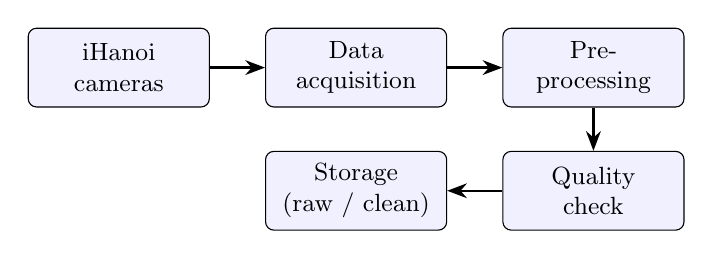
\begin{tikzpicture}[
  node distance=0.55cm and 0.7cm,
  box/.style={draw, rounded corners=3pt, minimum width=2.3cm, minimum height=1.0cm,
              align=center, font=\small, fill=blue!6},
  arr/.style={-{Stealth[length=2.5mm]}, thick}
]
  \node[box] (cam)  {iHanoi\\cameras};
  \node[box, right=of cam]  (acq)  {Data\\acquisition};
  \node[box, right=of acq]  (pre)  {Pre-\\processing};
  \node[box, below=of pre]  (qc)   {Quality\\check};
  \node[box, left=of qc]    (sto)  {Storage\\(raw / clean)};
  \draw[arr] (cam) -- (acq);
  \draw[arr] (acq) -- (pre);
  \draw[arr] (pre) -- (qc);
  \draw[arr] (qc)  -- (sto);
\end{tikzpicture}
\caption{Data preparation workflow.}
\label{fig:prep-flow}
\end{figure}

The acquisition component periodically retrieves data from the selected
cameras and stores it together with metadata. Its main design points are:
\begin{itemize}
  \item scheduled collection with a fixed sampling interval: the video stream
        of each camera is sampled at one frame per second (1~FPS), which is
        frequent enough to count vehicles and follow them across frames while
        keeping the data volume manageable;
  \item timeout and retry handling for unavailable cameras;
  \item each record saved with \texttt{camera\_id}, timestamp, and source URL;
  \item logging of failed requests for later quality analysis.
\end{itemize}

\subsection{Data Schema}
\label{subsec:schema}
The camera data is processed as video. For every frame, a vehicle detection
(and tracking, when available) step produces one record per detected vehicle.
Table~\ref{tab:schema} defines the output features.

\begin{table}[H]
\centering
\caption{Output features extracted from the camera video (one row per detected vehicle).}
\label{tab:schema}
\begin{tabularx}{\textwidth}{@{}l l X@{}}
\toprule
\textbf{Field} & \textbf{Type} & \textbf{Description} \\
\midrule
\texttt{detection\_id}  & string   & Unique identifier of the detection record \\
\texttt{camera\_id}     & string   & Identifier of the source camera \\
\texttt{timestamp}      & datetime & Time of the frame (UTC+7) \\
\texttt{frame\_index}   & int      & Frame order within the video \\
\texttt{vehicle\_id}    & string / null & Tracking ID if the vehicle can be followed across frames \\
\texttt{vehicle\_type}  & category & Car, motorcycle, bus, truck, etc. \\
\texttt{confidence}     & float    & Confidence score of the detection model \\
\texttt{bbox\_x1}, \texttt{bbox\_y1} & float & Top-left corner of the bounding box \\
\texttt{bbox\_x2}, \texttt{bbox\_y2} & float & Bottom-right corner of the bounding box \\
\texttt{bbox\_width}, \texttt{bbox\_height} & float & Width and height of the bounding box \\
\texttt{center\_x}, \texttt{center\_y} & float & Center of the vehicle in the frame \\
\texttt{vehicle\_area} & float & Bounding box area; may be normalized by the frame size \\
\bottomrule
\end{tabularx}
\end{table}

The fields \texttt{bbox\_width}, \texttt{bbox\_height}, \texttt{center\_x},
\texttt{center\_y}, and \texttt{vehicle\_area} are derived from
\texttt{bbox\_x1}, \texttt{bbox\_y1}, \texttt{bbox\_x2}, and \texttt{bbox\_y2}
and are computed during preprocessing to keep them consistent.

\subsection{Preprocessing}
\label{subsec:preprocessing}
Raw camera video is converted into clean detection records that follow the
schema in Table~\ref{tab:schema}. The preprocessing steps are:
\begin{enumerate}
  \item \textbf{Frame sampling:} extract frames from the video at 1~FPS and
        assign each frame a \texttt{frame\_index} and a \texttt{timestamp}
        (UTC+7).
  \item \textbf{Frame validation:} discard corrupted, black, and frozen frames.
  \item \textbf{Resizing:} resize frames to the input size of the detection
        model 640$\times$480.
  \item \textbf{Detection filtering:} keep only vehicle classes with
        \texttt{confidence} above a threshold 0.3, and remove
        invalid bounding boxes (outside the frame or with zero size).
  \item \textbf{Feature computation:} compute \texttt{bbox\_width},
        \texttt{bbox\_height}, \texttt{center\_x}, \texttt{center\_y}, and
        \texttt{vehicle\_area} from the box coordinates, and assign a
        \texttt{vehicle\_id} when the vehicle can be tracked (null otherwise).
\end{enumerate}

\subsection{Storage Layout}
\label{subsec:storage}
Data is stored in layers, from raw video to the final detection records. This
keeps the raw data unchanged and lets each stage be re-run independently.
Table~\ref{tab:storage} describes each layer.

\begin{lstlisting}
data/
  raw/
    videos/       <camera_id>/<YYYY>/<MM>/<DD>/<HHMMSS>.mp4
  frames/         <camera_id>/<YYYY>/<MM>/<DD>/<frame_index>.jpg
  detections/     camera_id=<camera_id>/date=<YYYY-MM-DD>/part-*.parquet
  logs/           acquisition_errors.log
\end{lstlisting}

\begin{table}[H]
\centering
\caption{Storage layers.}
\label{tab:storage}
\begin{tabularx}{\textwidth}{@{}l l X@{}}
\toprule
\textbf{Layer} & \textbf{Format} & \textbf{Content} \\
\midrule
\texttt{raw/videos}  & video MP4 & Original video segments, never modified \\
\texttt{frames}      & JPEG & Sampled and validated frames (kept for debugging and checking) \\
\texttt{detections}  & Parquet & Cleaned detection records following the schema in Table~\ref{tab:schema}, partitioned by camera and date \\
\texttt{logs}        & text & Failed requests, dropped videos, and dropped frames for quality analysis \\
\bottomrule
\end{tabularx}
\end{table}

% ============================================================
\section{Initial Results on Applying ML Models}
\label{sec:ml}

This section reports the first results of applying a machine learning model to
vehicle detection. The results are preliminary and are used to check that the
approach works before the full evaluation of the pipeline.

\subsection{Modeling Objective}
\label{subsec:ml-objective}
The first model addresses \textbf{vehicle detection and classification}: it
locates each vehicle in a frame with a bounding box and predicts its
\texttt{vehicle\_type} (car, motorcycle, bus, or truck) together with a
\texttt{confidence} score. These outputs are the inputs of the schema in
Table~\ref{tab:schema}. Vehicle tracking and the traffic indicators (vehicle
counts, density, and congestion level) are built on top of the detections and
are left for the next stage. Because the dataset used here is aerial imagery
and not iHanoi video, this experiment serves as a baseline for the detection
approach (see Section~\ref{subsec:ml-discussion}).

\subsection{Model Applied}
\label{subsec:ml-models}
We use \textbf{YOLO26s}, the small variant of the YOLO26 object detector, through
the Ultralytics framework (version 8.4.190). The model has about 9.5 million
parameters and 20.8 GFLOPs. It is initialized from pre-trained (COCO) weights
and fine-tuned for four classes: car, motorcycle, bus, and truck. The
pre-trained class head of the model is remapped to these four classes by class
name.

\subsection{Experimental Setup}
\label{subsec:ml-setup}
\begin{itemize}
  \item \textbf{Data:} the public dataset DLR-MVDA (DLR Multi-class Vehicle
        Detection and Orientation in Aerial Imagery) of the German Aerospace
        Center (DLR)~\cite{dlr-mvda}.
        It contains aerial images with annotated vehicles. The recorded iHanoi
        video does not yet have bounding-box labels, so this first experiment
        uses a labeled public dataset. The data was prepared in YOLO format
        with four classes (car, motorcycle, bus, truck), giving 534 images
        in total, split into 374 for training, 107 for validation, and 53 for
        testing (about 70/20/10). \todo{State how the original DLR annotations
        were converted to YOLO format and mapped to the four classes.}
  \item \textbf{Ground truth:} the vehicle bounding boxes and types annotated by
        the dataset authors (DLR).
  \item \textbf{Data split:} training (374 images, 750 vehicles), validation
        (107 images, 221 vehicles), and test (53 images, 97 vehicles). The
        results in this section are measured on the validation set; the test
        set has not been used yet.
  \item \textbf{Training:} up to 100 epochs, image size 640, batch size 16,
        AdamW optimizer (learning rate chosen automatically, 0.00125), with
        early stopping when the validation result does not improve for 20
        epochs.
  \item \textbf{Environment:} Google Colab with an NVIDIA Tesla T4 GPU.
\end{itemize}

\subsection{Evaluation Metrics}
\label{subsec:ml-metrics}
\begin{itemize}
  \item \textbf{Precision and recall:} the share of correct detections among
        all predicted vehicles, and the share of real vehicles that are found.
  \item \textbf{mAP@50:} mean average precision at an IoU threshold of 0.5.
  \item \textbf{mAP@50--95:} mean average precision averaged over IoU
        thresholds from 0.5 to 0.95, a stricter measure of box quality.
  \item \textbf{Inference speed:} time per image, because the pipeline must run
        in real time.
\end{itemize}
Counting error against manual counts is not evaluated yet and is planned for
the next stage.

\subsection{Results}
\label{subsec:ml-results}
Training stopped early after 21 epochs (about 0.12 hours), because the
validation result did not improve after the first epoch. The best model
(\texttt{best.pt}) was kept and evaluated on the validation set.
Table~\ref{tab:ml-results} shows the overall result and
Table~\ref{tab:ml-class} shows the result for each class.

\begin{table}[H]
\centering
\caption{Overall result of YOLO26s on the validation set (107 images, 221 vehicles).}
\label{tab:ml-results}
\begin{tabular}{@{}lrrrrr@{}}
\toprule
\textbf{Model} & \textbf{Precision} & \textbf{Recall} & \textbf{mAP@50} & \textbf{mAP@50--95} & \textbf{Inference} \\
\midrule
YOLO26s & 0.588 & 0.626 & 0.611 & 0.367 & 9.8 ms/image \\
\bottomrule
\end{tabular}
\end{table}

Including pre-processing (0.2~ms) and post-processing (1.5~ms), one image takes
about 11.5~ms on the T4 GPU, which is roughly 87 images per second. This is far
above the 1~FPS sampling rate used in Section~\ref{sec:data}.

\begin{table}[H]
\centering
\caption{Result of YOLO26s for each class on the validation set.}
\label{tab:ml-class}
\begin{tabular}{@{}lrrrrr@{}}
\toprule
\textbf{Class} & \textbf{Instances} & \textbf{Precision} & \textbf{Recall} & \textbf{mAP@50} & \textbf{mAP@50--95} \\
\midrule
Car        & 130 & 0.673 & 0.617 & 0.617 & 0.358 \\
Motorcycle &  29 & 0.454 & 0.517 & 0.455 & 0.194 \\
Bus        &  30 & 0.606 & 0.933 & 0.892 & 0.677 \\
Truck      &  32 & 0.619 & 0.438 & 0.480 & 0.239 \\
\midrule
All        & 221 & 0.588 & 0.626 & 0.611 & 0.367 \\
\bottomrule
\end{tabular}
\end{table}

Figure~\ref{fig:ml-curve} shows the validation result after each epoch.

\begin{figure}[H]
\centering
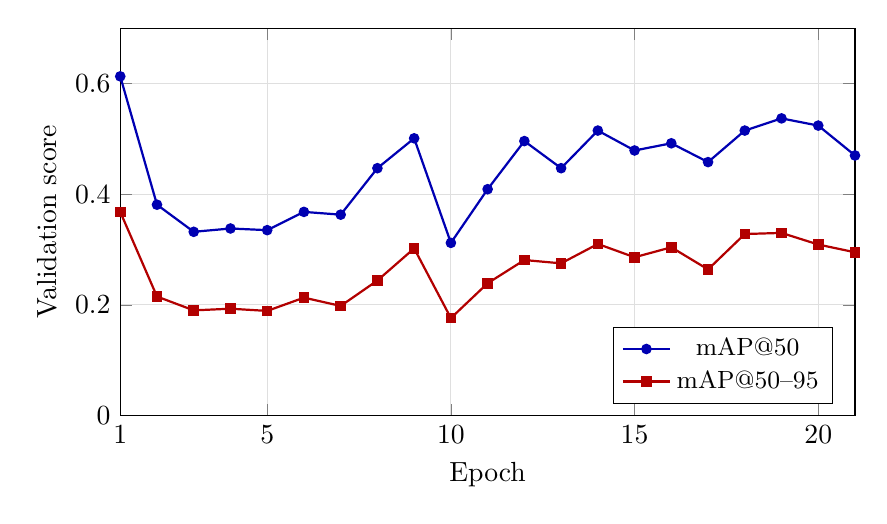
\begin{tikzpicture}
\begin{axis}[
  width=0.9\textwidth, height=6.5cm,
  xlabel={Epoch}, ylabel={Validation score},
  xmin=1, xmax=21, ymin=0, ymax=0.7,
  xtick={1,5,10,15,20},
  grid=major, grid style={gray!25},
  legend pos=south east, legend style={font=\small}
]
\addplot[blue!70!black, thick, mark=*, mark size=1.5pt] coordinates {
(1,0.613)(2,0.381)(3,0.332)(4,0.338)(5,0.335)(6,0.368)(7,0.363)(8,0.447)(9,0.501)(10,0.312)(11,0.409)
(12,0.496)(13,0.447)(14,0.515)(15,0.479)(16,0.492)(17,0.458)(18,0.515)(19,0.537)(20,0.524)(21,0.470)};
\addlegendentry{mAP@50}
\addplot[red!70!black, thick, mark=square*, mark size=1.5pt] coordinates {
(1,0.368)(2,0.215)(3,0.190)(4,0.193)(5,0.189)(6,0.213)(7,0.198)(8,0.244)(9,0.302)(10,0.176)(11,0.239)
(12,0.281)(13,0.275)(14,0.310)(15,0.286)(16,0.304)(17,0.264)(18,0.328)(19,0.330)(20,0.309)(21,0.295)};
\addlegendentry{mAP@50--95}
\end{axis}
\end{tikzpicture}
\caption{Validation mAP of YOLO26s after each training epoch.}
\label{fig:ml-curve}
\end{figure}

\subsection{Discussion}
\label{subsec:ml-discussion}
\paragraph{Overall.}
YOLO26s reaches mAP@50 of 0.611 and recall of 0.626 on the validation set, so
the model already finds a large part of the vehicles. The precision of 0.588 and
the mAP@50--95 of 0.367 show that many boxes are still inaccurate or wrong.
The result is a first baseline, not yet good enough for reliable counting.

\paragraph{Per class.}
Buses are detected best (mAP@50 of 0.892, recall of 0.933), which is expected
because they are large and visually distinct. Motorcycles are the weakest class
(mAP@50 of 0.455, mAP@50--95 of 0.194). A likely reason is that motorcycles appear
very small in the images and are often close together; this should be checked
on example frames. Trucks have the lowest recall (0.438), meaning more than half of
them are missed; they may be confused with cars or buses. Cars, the largest
class with 130 instances, reach a middle level (mAP@50 of 0.617).

\paragraph{Domain difference.}
DLR-MVDA consists of aerial images taken from above, while the iHanoi cameras
are roadside cameras with an oblique view, where vehicles look very different
(shape, size, occlusion). A model trained only on aerial images is therefore
not expected to reach the same accuracy on iHanoi frames. The results above
show that the approach and the training procedure work, but they do not yet
measure the performance on the target data.

\paragraph{Training behavior.}
The best validation result appears at the \emph{first} epoch (mAP@50 of 0.613,
mAP@50--95 of 0.368). It then drops sharply and stays unstable, between 0.19 and
0.33 for mAP@50--95, and never exceeds the first epoch. At the same time the
training loss keeps decreasing, while the validation classification loss does
not improve. This suggests that the model quickly adapts to the small training
set while the pre-trained weights already give a good starting point, and
further training does not generalize. The cause still needs to be investigated.

\subsection{Limitations and Next Steps}
\label{subsec:ml-next}
The current results have the following limitations:
\begin{itemize}
  \item the dataset is small (534 images), and the classes are imbalanced
        (462 cars against fewer than 100 instances for each other class in
        the training set);
  \item the training data is aerial imagery, not iHanoi camera video, so the
        results do not directly describe the performance of the pipeline on
        its target data;
  \item the reported results are measured on the validation set, which was also
        used to choose the best model, so they may be optimistic; the test set
        (53 images) has not been evaluated yet;
  \item the result comes from a single training run, and the training was
        unstable;
  \item counting error and tracking have not been evaluated yet.
\end{itemize}
The planned next steps are:
\begin{itemize}
  \item investigate the unstable training (e.g., a lower learning rate, a
        warm-up period, stronger data augmentation) and train again;
  \item add more data, especially for motorcycles and trucks;
  \item evaluate the final model once on the test set;
  \item evaluate the model on frames from the iHanoi cameras, and annotate a
        small set of iHanoi frames to fine-tune and test the model;
  \item add vehicle tracking and compute vehicle counts, then compare them with
        manual counts;
  \item connect the best model to the real-time pipeline.
\end{itemize}

% ============================================================
% Future sections (to be added part by part)
% ============================================================
% \section{Real-Time Streaming Architecture}
% \section{Evaluation}
% \section{Conclusion}

\clearpage
\addcontentsline{toc}{section}{References}
\begin{thebibliography}{9}
\bibitem{dlr-mvda} German Aerospace Center (DLR), Remote Sensing Technology
  Institute. \emph{DLR Multi-class Vehicle Detection and Orientation in Aerial
  Imagery (DLR-MVDA)}. Accessed 10 November 2026. \\
  Page: \url{https://www.dlr.de/en/eoc/about-us/remote-sensing-technology-institute/photogrammetry-and-image-analysis/public-datasets/dlr-mvda} \\
  Download: \url{https://pba-freesoftware.eoc.dlr.de/MunichDatasetVehicleDetection-2015-old.zip}
\end{thebibliography}

\end{document}